%
% 6.006 problem set 4 solutions template
%
\documentclass[12pt,twoside]{article}

\usepackage{amsmath}
\usepackage{color}
\usepackage{tikz}

\input{macros}

\setlength{\oddsidemargin}{0pt}
\setlength{\evensidemargin}{0pt}
\setlength{\textwidth}{6.5in}
\setlength{\topmargin}{0in}
\setlength{\textheight}{8.5in}

\newcommand{\theproblemsetnum}{4}
\newcommand{\releasedate}{Wednesday, November 2, 2016}
\newcommand{\partaduedate}{Tuesday, November 15, 2016}
\newcommand{\tabUnit}{3ex}
\newcommand{\tabT}{\hspace*{\tabUnit}}

\title{6.006 Problem Set 4}

\begin{document}

\handout{Problem Set \theproblemsetnum}{Wednesday, November 2, 2016}

\textbf{All parts are due {\bf \partaduedate} at {\bf 11:59PM}}.

\setlength{\parindent}{0pt}

\medskip

\hrulefill

\medskip

{\bf Name:} Milo Knowles

\medskip

{\bf Collaborators:}

\medskip

\hrulefill

%%%%%%%%%%%%%%%%%%%%%%%%%%%%%%%%%%%%%%%%%%%%%%%%%%%%%
% See below for common and useful latex constructs. %
%%%%%%%%%%%%%%%%%%%%%%%%%%%%%%%%%%%%%%%%%%%%%%%%%%%%%

% Some useful commands:
%$f(x) = \Theta(x)$
%$T(x, y) \leq \log(x) + 2^y + \binom{2n}{n}$
% {\tt code\_function}


% You can create unnumbered lists as follows:
%\begin{itemize}
%    \item First item in a list 
%        \begin{itemize}
%            \item First item in a list 
%                \begin{itemize}
%                    \item First item in a list 
%                    \item Second item in a list 
%                \end{itemize}
%            \item Second item in a list 
%        \end{itemize}
%    \item Second item in a list 
%\end{itemize}

% You can create numbered lists as follows:
%\begin{enumerate}
%    \item First item in a list 
%    \item Second item in a list 
%    \item Third item in a list
%\end{enumerate}

% You can write aligned equations as follows:
%\begin{align} 
%    \begin{split}
%        (x+y)^3 &= (x+y)^2(x+y) \\
%                &= (x^2+2xy+y^2)(x+y) \\
%                &= (x^3+2x^2y+xy^2) + (x^2y+2xy^2+y^3) \\
%                &= x^3+3x^2y+3xy^2+y^3
%    \end{split}                                 
%\end{align}

% You can create grids/matrices as follows:
%\begin{align}
%    A = 
%    \begin{bmatrix}
%        A_{11} & A_{21} \\
%        A_{21} & A_{22}
%    \end{bmatrix}
%\end{align}

\begin{problems}

\section*{Part A}

\problem  % Problem 1

\begin{problemparts}
\problempart Make the weight of every edge the weight of the node it leads into. Then, remove the weights from all the nodes. Now, we have an edge weighted graph, and every path will still have the same cost as in the node-weighted case. Edges that go into a node with no weight (i.e Base B) will simply have no weight. For example, if we modified the example from Problem 1:

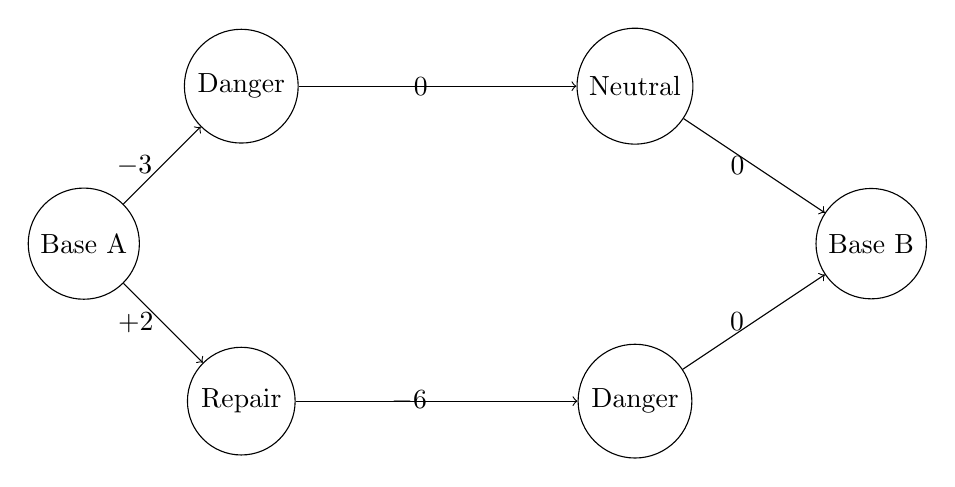
\begin{tikzpicture}
	\node[shape=circle,draw=black] (A) at (0,0) {Base A};
	\node[shape=circle,draw=black] (B) at (2,2) {Danger};
	\node[shape=circle,draw=black] (C) at (7,2) {Neutral};
	\node[shape=circle,draw=black] (D) at (10,0) {Base B};
	\node[shape=circle,draw=black] (E) at (2,-2) {Repair};
	\node[shape=circle,draw=black] (F) at (7,-2) {Danger};

	\path [->](A) edge node[left] {$-3$} (B);
	\path [->](B) edge node[left] {$0$} (C);
	\path [->](C) edge node[left] {$0$} (D);
	\path [->](A) edge node[left] {$+2$} (E);
	\path [->](E) edge node[left] {$-6$} (F);
	\path [->](F) edge node[left] {$0$} (D);
\end{tikzpicture}


\problempart The total cost of a path represents the net change in integrity of Speedy's armor, which we can call $D$. In order for Speedy to successfully complete a mission, 

$C+D \geq 0$
$\implies D \geq - C$

\smallskip
If this is true, then Speedy can complete the mission, because his armor integrity will be $\geq 0 $ when he reaches his destination.

We can adapt the Bellman-Ford algorithm to find a single-source shortest path from Base A to Base B on our network of roads. However, in this case our "shortest path" is the path that maximizes the weight of the path (this is best for Speedy. To adapt Bellman Ford to do this, we initialize all of our nodes with a weight of negative infinity, and change our relaxation function to the following for two vertices $u$ and $v$. \\

if $v.d + w_{uv} > u.d$:\\
then $u.d = v.d + w_{uv}$\\

Assuming there are no positive-weight cycles, Bellman-Ford can find a best in $O(VE)$ time, because it requires $\abs{V} - 1$ rounds of edge relaxation over $E$ edges to find the shortest path. If the weight of the best path is $\geq -C$, then we know that Speedy can complete his mission.

\problempart Speedy is caught in a positive-weight cycle. Because Speedy is still traversing the graph, but his armor integrity has not dropped below 0, this is the only possibility. An example graph looks like the following:

\begin{tikzpicture}
	\node[shape=circle,draw=black] (A) at (0,0) {Base A};
	\node[shape=circle,draw=black] (B) at (2,2) {B};
	\node[shape=circle,draw=black] (C) at (7,2) {C};
	\node[shape=circle,draw=black] (D) at (10,0) {Base B};
	\node[shape=circle,draw=black] (E) at (2,-2) {D};
	\node[shape=circle,draw=black] (F) at (7,-2) {E};
	\node[shape=circle,draw=black] (G) at (7,5) {F};
	\node[shape=circle,draw=black] (H) at (10,3) {G};

	\path [->](A) edge node[left] {$-3$} (B);
	\path [->](B) edge node[left] {$0$} (C);
	\path [->](C) edge node[left] {$0$} (D);
	\path [->](A) edge node[left] {$+2$} (E);
	\path [->](E) edge node[left] {$-6$} (F);
	\path [->](F) edge node[left] {$0$} (D);
	\path [->](C) edge node[left] {$1$} (G);
	\path [->](G) edge node[left] {$4$} (H);
	\path [->](H) edge node[left] {$2$} (C);
\end{tikzpicture}

In this case, if Speedy arrives at vertex C, he will enter a never-ending loop from C to F to G to C, increasing his armor integrity with each cycle. He will never reach Base B because he will always be able to improve his armor by going around the cycle.

\problempart Similar to Part B, we can use an adapted version of the Bellman Ford algorithm to find the highest-weight path to every node in the graph. We can start at any arbitrary Normally, the algorithm will find the highest-weight path to every node in $\abs{V}-1$ iterations. However, if on the $Vth$ iteration we can still perform relaxations on on the graph and the highest weight of vertices continues to increase, this means that there must be positive-weight cycles in the graph. 

If there is a positive weight cycle, any node that is reachable from that positive weight cycle will continue to increase it's weight as Bellman-Ford runs. On the $Vth$ iteration of Bellman-Ford, start storing all of 

\end{problemparts}

\problem  % Problem 2

\begin{problemparts}
\problempart

In order to ensure that Jerry's path ends up at a hiding spot on every 3rd move, we create a graph $G_3$, which is a triple copy of $G$. Each vertex $v$ in $G$ has 3 vertices in $G_3$: $v_1$, $v_2$, and $v_3$. For every edge $(u, v)$ in the original graph, create the edges $(u_1, v_2)$, $(u_2, v_3)$, and $(u_3, v_1)$. This will take $O(V + E)$ time, because we are creating $2V$ extra vertices, and $2E$ extra edges. The structure of $G_3$ ensures that, if Jerry starts at some vertex with a subscript 1, he will end up at another vertex with subscript 1 in three moves.

Remove every vertex with subscript 1 from $G_3$ that is not a hiding spot. Now, every path that exists from $s_1$ to $f_1$ is guaranteed to end up at a hiding spot on every 3rd move. This takes $O(h)$ time, where $h$ is the number of hiding spots (guaranteed to be $O(V)$). 

Jerry can only move North or East in this X by Y graph, so there cannot be any cycles. Therefore, this is a Directed-Acyclic-Graph. We can find a single-source-shortest-path on a DAG in $O(V+E)$ time by topologically sorting our graph $G$ and then doing one iteration of Bellman-Ford, relaxing nodes in the order of the topological sort. Run Bellman-Ford to find the shortest path from $s_1$ to $f_1$ in $G_3$. This path will require the least effort, and guarantee that Jerry ends up at a hiding spot every 3rd minute.

The runtime of this algorithm is $O(V+E)$, because we add up the $O(V+E)$ time to create our augmented graph, $O(V)$ time to remove non-hiding spots, and $O(V+E)$ time to run Bellman-Ford on our DAG.


\problempart 

Similar to Part A, we create an augmented version $G_3(V, E, w)$ of our graph $G(V, E, w)$. First, create self-loops of weight zero for every vertex in $G$. Then, for each vertex $v$ in $G$, create 3 vertices in $G_3$: $v_1$, $v_2$, and $v_3$. For every edge $(u, v)$ in the original graph, create the edges $(u_1, v_2)$, $(u_2, v_3)$, and $(u_3, v_1)$ in $G_3$. 

Remove every vertex with subscript 1 from $G_3$ that is not a hiding spot. Now, every path that exists from $s_1$ to $f_1$ is guaranteed to traverse at most 3 edges between hiding spots, and takes into account the fact that Jerry can wait at any vertex. Creating our augmented graph $G_3$ takes $O(V+E)$ time, because it adds $2V$ vertices and $3E$ edges, and removes $O(V)$ vertices.

Use Dijkstra's Algorithm on $G_3$ in $O(V\log V + E)$ time using a Fibonacci heap. Dijkstra's Algorithm works for weighted graphs with cycles, so we are fine.

The algorithm takes $O(V + E)$ time to build our augmented graph, and $O(V\log V + E)$ time to find the shortest path on it. Therefore, the overall runtime is $O(V\log V + E)$.

\end{problemparts}

\problem  % Problem 3

\begin{problemparts}
\problempart Part a % Problem 3a
\problempart Part b % Problem 3b
\end{problemparts}

\section*{Part B}

\problem
\begin{problemparts}
\problempart \emph{Submit your implementation on alg.csail.mit.edu}
\problempart \emph{Submit your implementation on alg.csail.mit.edu}
\end{problemparts}

\end{problems}

\end{document}

